\section{Experimental Results}
\label{chap:experiments}
This chapter presents the empirical findings from the comparative experiments conducted according to the fair benchmarking framework and methodology detailed in Chapter~\ref{chap:methodology}. The results focus on evaluating the performance and energy efficiency of the alternative algorithms against their respective fair backpropagation (BP) baselines across the MNIST, Fashion-MNIST, CIFAR-10, and CIFAR-100 datasets.

Although performance is primarily assessed through the accuracy of classification and convergence behavior, efficiency evaluation utilizes a multifaceted approach. To provide a robust assessment of practical computational and energy efficiency, the analysis prioritizes directly measured hardware metrics. These primary indicators include total energy consumption, measured in Watt-hours (Wh) using the NVML API, the wall-clock training time until termination by early stopping, and the peak GPU memory usage, also monitored via NVML. These measurements reflect the utilization of real-world resources on the specified NVIDIA A100 hardware platform. To supplement these hardware-specific metrics, estimated GFLOPs for a single forward pass ($F_{fwd}$), obtained using the PyTorch Profiler, are reported to provide a hardware-agnostic measure of arithmetic complexity. For BP baselines, the estimated GFLOPs per update cycle ($F_{BP\_update} \approx 3 \times F_{fwd}$) are included to illustrate the theoretical computational difference that arises from the backward pass. Furthermore, an estimated CO2e is reported, calculated to provide an environmental impact perspective based on the measured energy consumption within the specified compute region (Poland, ISO code: POL). The subsequent sections detail the results for each algorithm and its corresponding baseline, followed by comparative analyzes focusing on these key performance and efficiency indicators.

\subsection{Forward-Forward (FF) vs. Backpropagation (BP) Comparison}
\label{sec:exp_ff_vs_bp}
This section presents a foundational analysis comparing Geoffrey Hinton's FF algorithm against a fair BP baseline, focusing on the MLP architectures for which FF was primarily designed. The initial performance results reveal a significant paradox: while FF can achieve impressive accuracy, thus validating its core concept, it does so at a drastically higher convergence cost.

\begin{table}[htbp]
    \centering
    \caption{Performance Comparison: FF vs. BP on MLP Architectures (Mean ± Std Dev over 3 runs).}
    \label{tab:ff_bp_mlp_perf_results_ch4}
    \begin{tabular}{lll c c}
        \toprule
        Dataset & Architecture & Algorithm & Test Accuracy (\%) & Effective Epochs \\
        \midrule
        \multirow{2}{*}{F-MNIST} & \multirow{2}{*}{4 $\times$ 2000 MLP} & FF-AdamW & \textbf{89.63 ± 0.12} & 90.33 ± 16.86 \\
         & & BP Baseline& 88.88 ± 0.61 & \textbf{15.67 ± 0.58} \\
        \midrule
        \multirow{3}{*}{MNIST} & \multirow{3}{*}{3 $\times$ 1000 MLP} & FF-AdamW & \textbf{98.33 ± 0.03} & 77.00 ± 0.00 \\
         & & FF-SGD & 98.23 ± 0.05 & 99.33 ± 1.15 \\
         & & BP Baseline & 98.09 ± 0.06 & \textbf{35.00 ± 0.00} \\
        \midrule
        \multirow{2}{*}{MNIST} & \multirow{2}{*}{4 $\times$ 2000 MLP} & FF-AdamW & 98.42 ± 0.14 & 87.00 ± 11.53 \\
         & & BP Baseline & \textbf{98.43 ± 0.03} & \textbf{49.00 ± 0.00} \\
        \bottomrule
    \end{tabular}
    \caption*{\footnotesize Effective Epochs: Average number of global training epochs completed before early stopping. Best results in each comparison group are highlighted in \textbf{bold}. For accuracy, higher is better; for epochs, lower is better.}
\end{table}

As shown in Table~\ref{tab:ff_bp_mlp_perf_results_ch4}, the FF algorithm successfully trains MLP architectures to a final test accuracy that is competitive with, and in some cases slightly superior to, a fairly tuned BP baseline on both the MNIST and Fashion-MNIST datasets.  This result is significant, as it validates the core premise of Hinton's work: effective learning is indeed possible without propagating error gradients backwards.

However, the Effective Epochs metric in Table~\ref{tab:ff_bp_mlp_perf_results_ch4} reveals the steep cost of this accuracy. FF consistently required a dramatically higher number of training epochs to reach its optimal validation checkpoint, often more than double that of BP, indicating a far less efficient learning process. The practical implications of this inefficiency are best understood by analyzing the convergence behavior with respect to the actual wall-clock time.

\begin{figure}[htbp] 
    \centering
    \begin{subfigure}{0.85\textwidth}
        \centering
        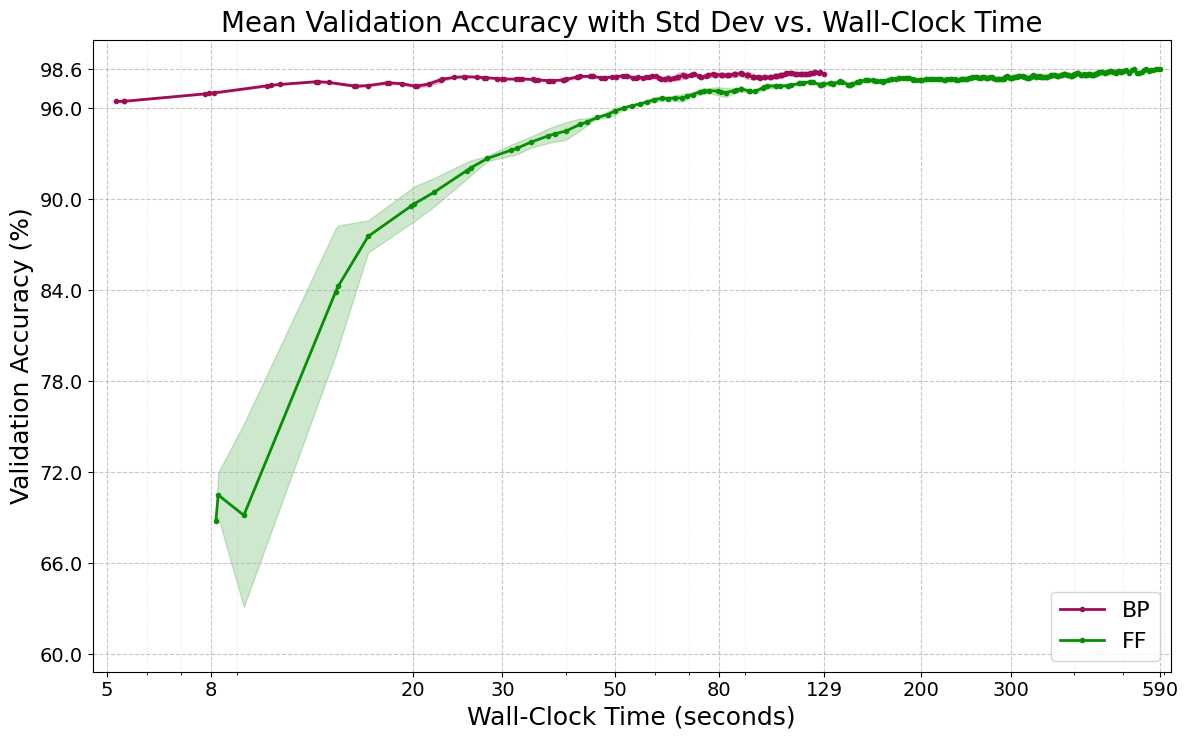
\includegraphics[width=\linewidth]{plots/FF_1.png}
        \caption{}
        \label{fig:ch4_ff_bp_mnist_mlp_4x2000_val_acc_time}
    \end{subfigure}
    \hfill
    \begin{subfigure}{0.85\textwidth}
        \centering
        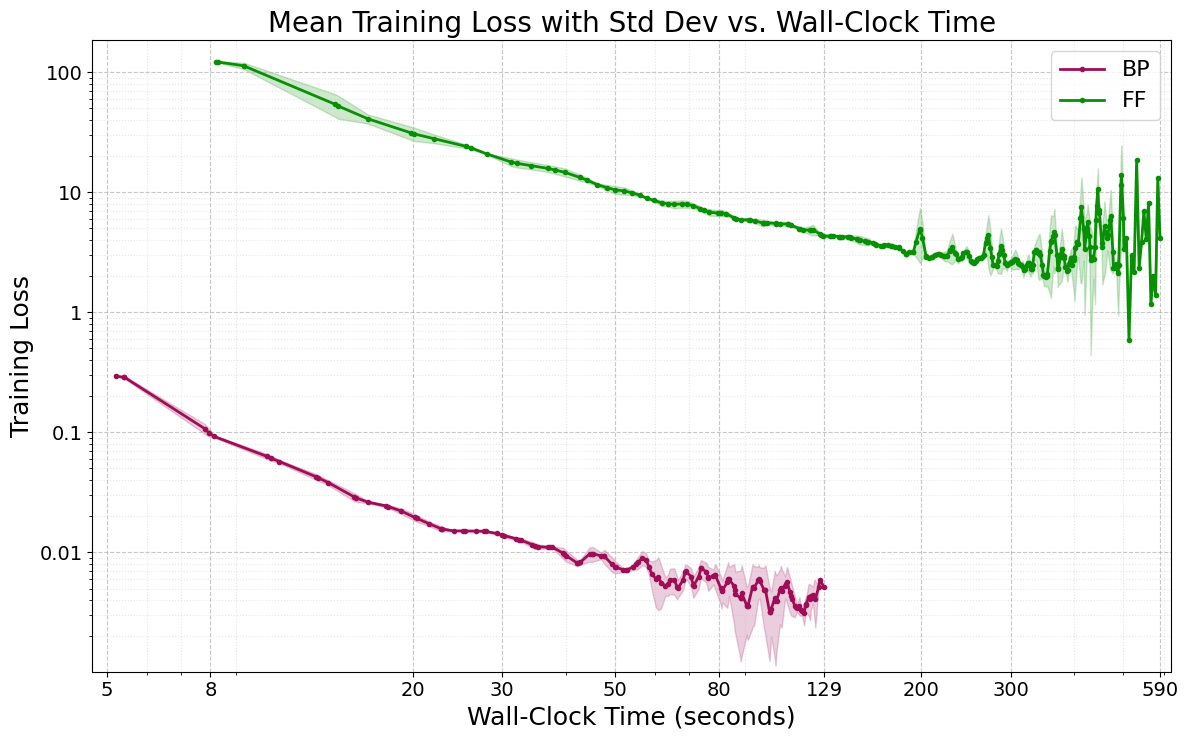
\includegraphics[width=\linewidth]{plots/FF_2.png}
        \caption{}
        \label{fig:ch4_ff_bp_mnist_mlp_4x2000_train_loss_time}
    \end{subfigure}
    \caption{Convergence Dynamics for FF vs. BP on MNIST 4 $\times$ 2000 MLP.}
    \label{fig:ch4_ff_bp_mnist_mlp_4x2000_conv_time}
\end{figure}

Figure~\ref{fig:ch4_ff_bp_mnist_mlp_4x2000_conv_time} provides a clear representation of this inefficiency. The validation accuracy plot (Figure~\ref{fig:ch4_ff_bp_mnist_mlp_4x2000_val_acc_time}) shows that the BP baseline achieves near-optimal performance rapidly, in well under 100 seconds, with a stable and consistent learning trajectory. In stark contrast, FF embarks on a slow, gradual, and more volatile learning path, which requires more than 400 seconds to reach a similar accuracy level. The training loss plot (Figure~\ref{fig:ch4_ff_bp_mnist_mlp_4x2000_train_loss_time}) reveals the underlying algorithmic cause for this disparity: BP's loss decreases smoothly and efficiently, whereas FF's loss decreases slowly and erratically from a much higher starting point, ultimately plateauing at a level orders of magnitude above that of BP. This indicates that FF's collection of local "goodness" objectives serves as a far weaker and less direct proxy for the global classification task, resulting in a fundamentally less efficient optimization landscape that necessitates a protracted training process with severe consequences for overall resource consumption.

The slow convergence of the FF algorithm directly translates into a significant increase in computational cost across all measured efficiency metrics. As detailed in Table~\ref{tab:ff_bp_mlp_eff_results_ch4}, the training time required to reach the best model was substantially longer (a 4x to 13x increase) and the total energy consumption was significantly higher (a 3x to 10x increase) for FF compared to BP across all configurations. This led to a correspondingly larger estimated CO2e footprint. 

\begin{table}[htbp]
    \centering
    \caption{Efficiency Comparison: FF vs. BP on MLP Architectures (Mean ± Std Dev over 3 runs).}
    \label{tab:ff_bp_mlp_eff_results_ch4}
    \resizebox{\textwidth}{!}{%
    \begin{tabular}{ccc c@{ ± }c c@{ ± }c c@{ ± }c c c}
        \toprule
        Dataset & Architecture & Algorithm & \multicolumn{2}{c}{Train Time (s)} & \multicolumn{2}{c}{Energy (Wh)} & \multicolumn{2}{c}{Est. CO2e (g)} & Peak Mem (MiB) & Total GFLOPs \\
        \midrule
        \multirow{2}{*}{F-MNIST} & \multirow{2}{*}{4 $\times$ 2000 MLP} & FF-AdamW & 574.60 & 134.49 & 14.28 & 2.66 & 23.10 & 8.52 & 1190 & \textbf{0.027} \\
        & & BP Baseline & \textbf{43.09} & \textbf{0.80} & \textbf{1.48} & \textbf{0.01} & \textbf{1.67} & \textbf{0.01} & \textbf{1168} & 0.082 \\
        \midrule
        \multirow{3}{*}{MNIST} & \multirow{3}{*}{3 $\times$ 1000 MLP} & FF-AdamW & 370.72 & 8.63 & 6.68 & 0.30 & 10.44 & 0.82 & 954 & \textbf{0.006} \\
        & & FF-SGD & 444.15 & 5.07 & 7.89 & 0.16 & 12.26 & 0.73 & 956 & \textbf{0.006} \\
        & & BP Baseline& \textbf{83.85} & \textbf{1.12} & \textbf{1.52} & \textbf{0.01} & \textbf{2.55} & \textbf{0.29} & \textbf{946} & 0.017 \\
        \midrule
        \multirow{2}{*}{MNIST} & \multirow{2}{*}{4 $\times$ 2000 MLP} & FF-AdamW & 509.59 & 73.20 & 14.26 & 1.74 & 17.50 & 2.74 & 1190 & \textbf{0.027} \\
        & & BP Baseline & \textbf{125.80} & \textbf{3.13} & \textbf{4.23} & \textbf{0.11} & \textbf{5.25} & \textbf{0.07} & \textbf{1168} & 0.082 \\
        \bottomrule
    \end{tabular}%
    }
    \caption*{\footnotesize Total GFLOPs: Estimated GigaFLOPs per sample. For FF, this is the cost of a single forward pass ($F_{fwd}$). For BP, it is the estimated cost of a full update cycle ($F_{BP\_update}$). Best efficiency results in each comparison group are highlighted in \textbf{bold} (lower is better).}
\end{table}

A definitive explanation for this inefficiency emerges from an analysis of the hardware-level monitoring plots in Figure~\ref{fig:ch4_ff_bp_mnist_mlp_4x2000_resource_util}. The memory plot (Figure~\ref{fig:ch4_ff_bp_mnist_mlp_4x2000_proc_mem_time}) reveals a critical and counterintuitive finding: contrary to the theoretical benefit of avoiding activation storage, \textbf{the FF algorithm consistently used slightly more GPU peak memory than BP in these experiments}. This observation empirically refutes a key presumed advantage, suggesting that practical implementation overheads, such as managing separate local optimizers, handling positive and negative data streams, or other specific PyTorch implementation details, impose a memory cost that outweighs the theoretical savings for these MLPs. More revealing is the GPU SM clock speed plot (Figure~\ref{fig:ch4_ff_bp_mnist_mlp_4x2000_sm_clock_time}), which provides a clear indicator of FF's inefficiency. While BP maintains a high, stable GPU clock speed, indicating that it effectively saturates the hardware with large, parallelizable matrix multiplications, FF's clock speed is erratic, "spiky," and operates at a lower average. This pattern signifies a computational bottleneck in which the GPU is frequently stalled, likely due to a high volume of small, sequential operations that lead to poor hardware utilization. Consequently, \textbf{FF's slowness is not due to its computations being inherently more complex, but to its failure to efficiently utilize modern, highly parallel hardware}.

\begin{figure}[htbp]
    \centering
    \begin{subfigure}{1.0\textwidth}
        \centering
        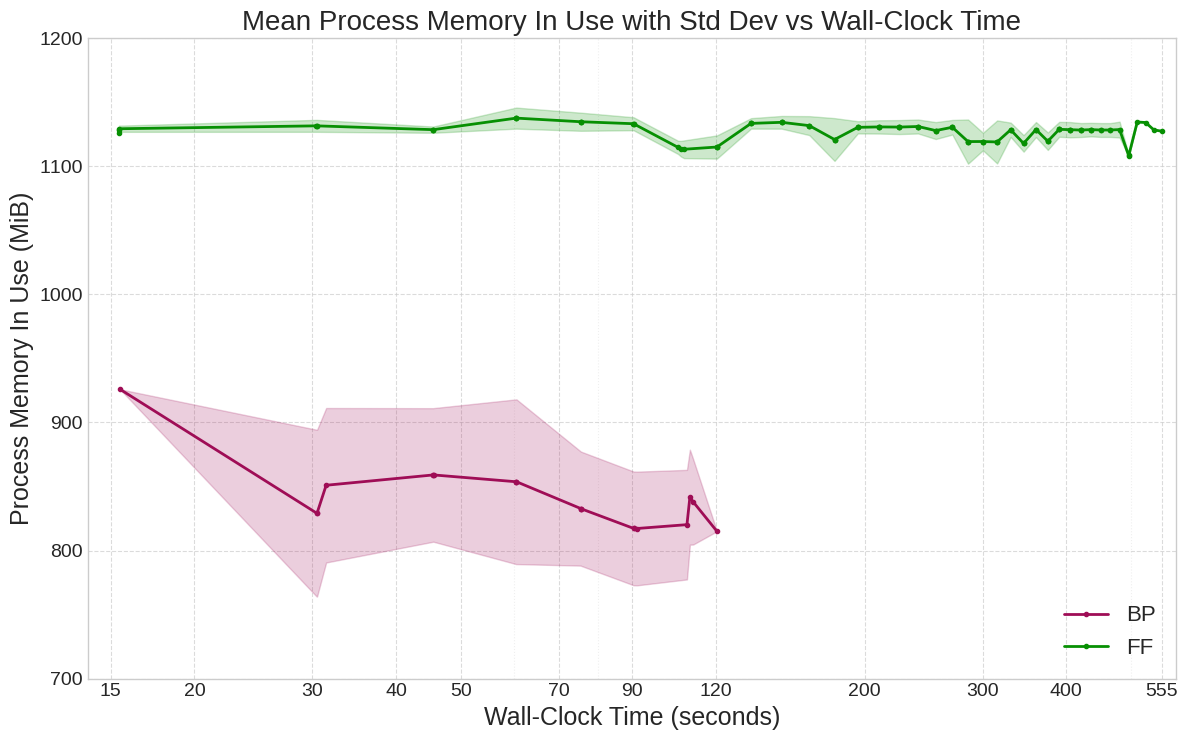
\includegraphics[width=\linewidth]{plots/FF_4.png}
        \caption{}
        \label{fig:ch4_ff_bp_mnist_mlp_4x2000_proc_mem_time}
    \end{subfigure}
    \hfill
    \begin{subfigure}{1.0\textwidth}
        \centering
        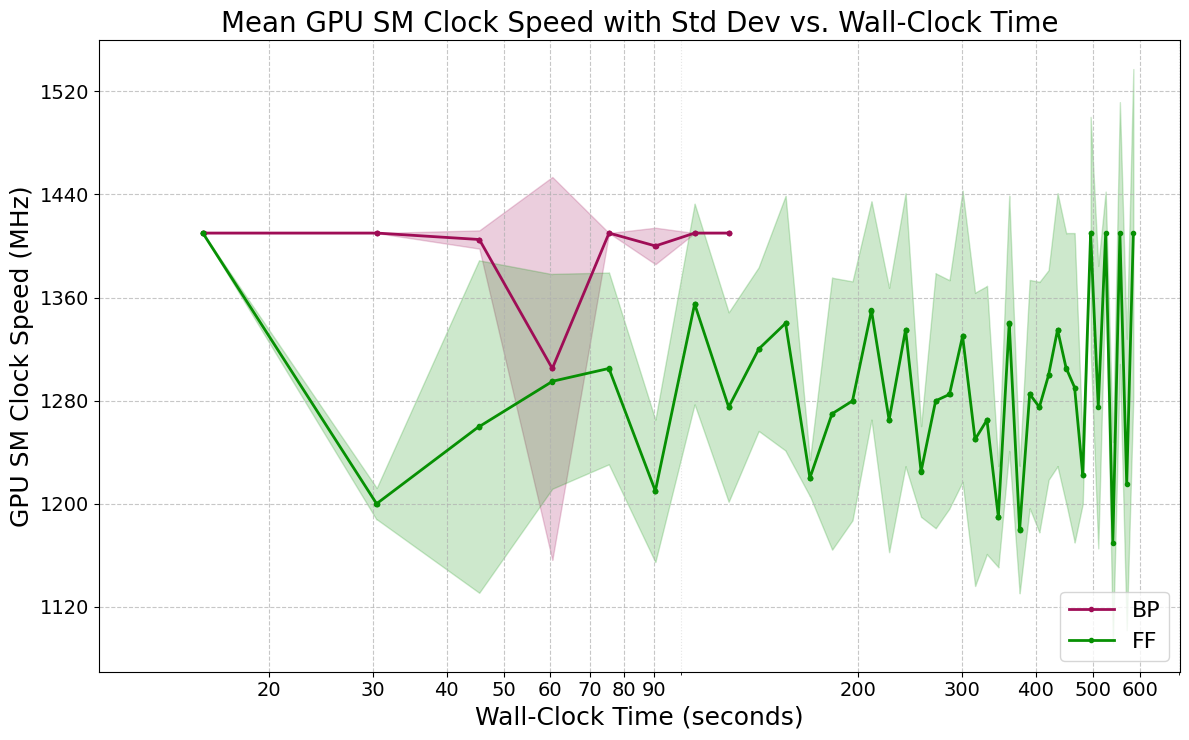
\includegraphics[width=\linewidth]{plots/FF_5.png}
        \caption{}
        \label{fig:ch4_ff_bp_mnist_mlp_4x2000_sm_clock_time}
    \end{subfigure}
    \caption{GPU Resource Utilization Profiles for FF vs. BP on MNIST 4 $\times$ 2000 MLP.}
    \label{fig:ch4_ff_bp_mnist_mlp_4x2000_resource_util}
\end{figure}

\textbf{In summary}, the FF algorithm serves as a vital foundational exploration, confirming its conceptual validity by training MLP architectures to an accuracy competitive with backpropagation. However, this success comes at a severe and disproportionate efficiency cost. The combination of a less effective optimization process and inefficient hardware utilization results in drastically longer training times, higher energy consumption, and a larger estimated CO2e footprint, while theoretical memory savings were not realized in this practical context. These findings quantify FF's shortcomings and motivate the investigation of more structured approaches like CaFo, which aim to resolve these inefficiencies by integrating supervisory signals more directly.

\subsection{Cascaded-Forward (CaFo) vs. Backpropagation (BP) Comparison}
\label{sec:exp_cafo_vs_bp_ch4}

This section presents a holistic analysis of the CaFo algorithm on its native 3-block CNN architecture, moving beyond foundational concepts to evaluate its practical viability as a structured BP-free alternative. The investigation covers two primary variants, CaFo-Rand-CE (using randomly initialized, fixed blocks) and CaFo-DFA-CE (using blocks pre-trained with DFA), against a fair BP baseline. By integrating dynamic convergence behavior with final, static performance, and efficiency metrics, a complete picture of the algorithm's inherent trade-offs is constructed. To understand CaFo's practical efficiency, it is crucial to first analyze the distinct convergence behaviors of its different variants.

\begin{figure}[htbp]
    \centering
    \begin{subfigure}{0.80\textwidth}
        \centering
        \includegraphics[width=\linewidth]{plots/Cafo_2.png}
        \label{fig:ch4_cafo_bp_fmnist_cnn_val_acc_time_reordered}
    \end{subfigure}
    \hfill
    \begin{subfigure}{0.80\textwidth}
        \centering
        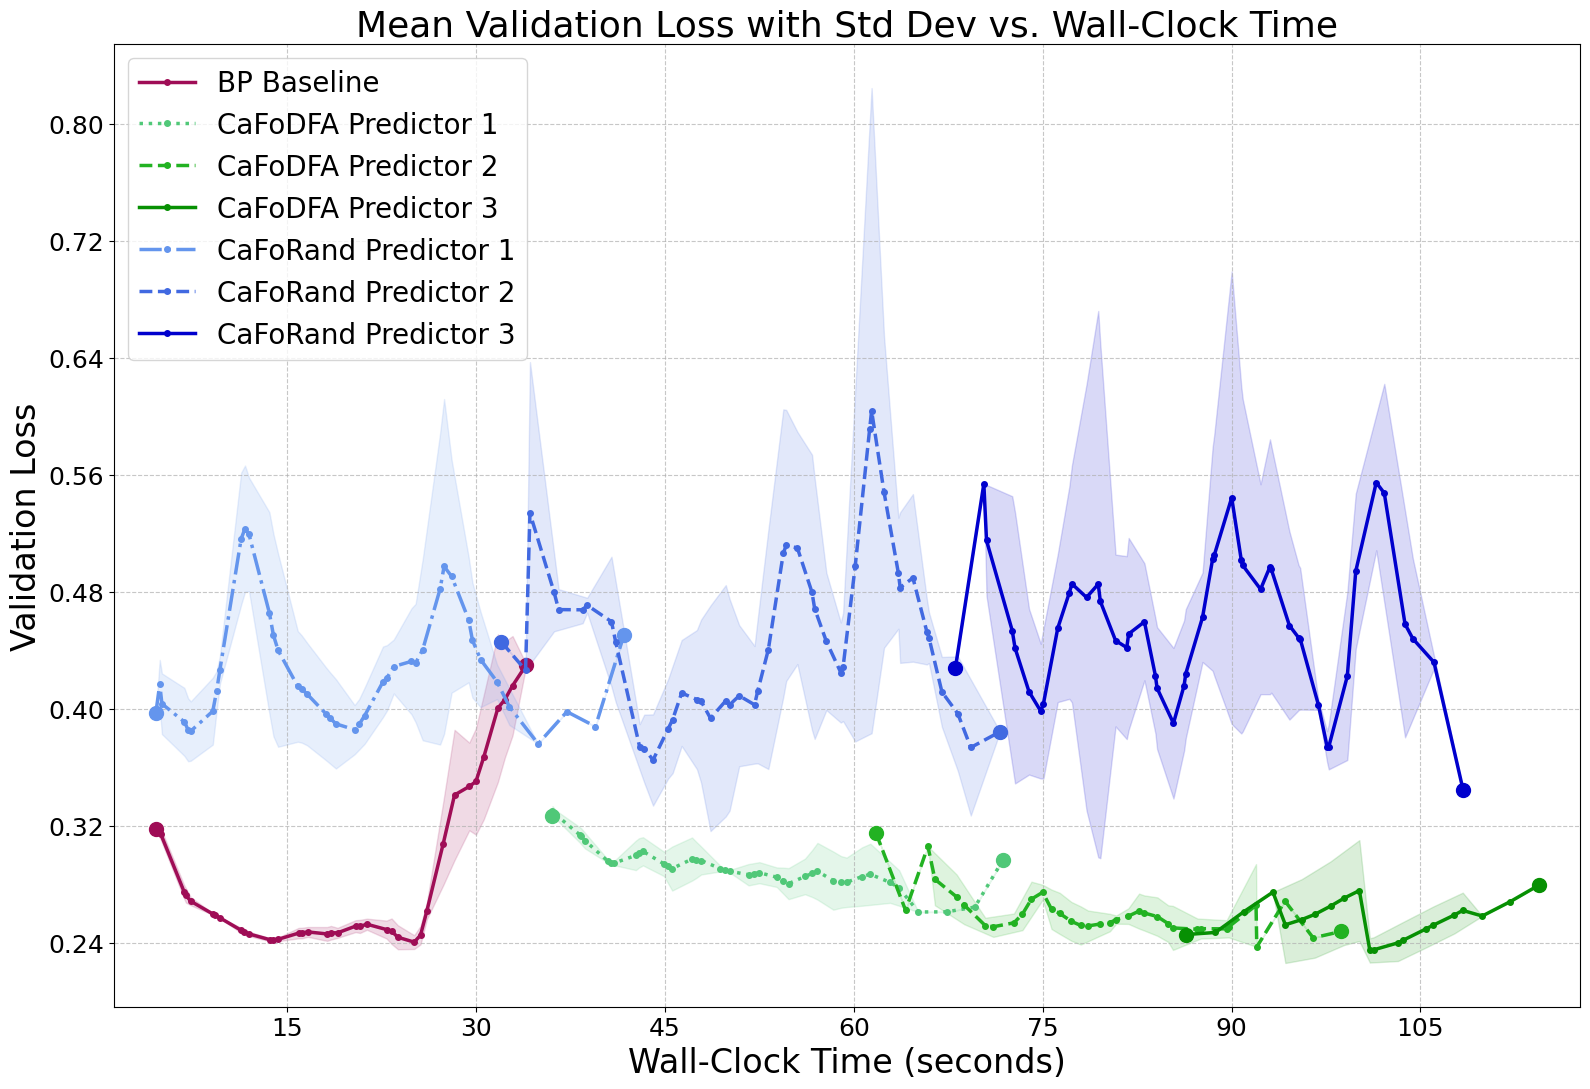
\includegraphics[width=\linewidth]{plots/Cafo_1.png}
        \label{fig:ch4_cafo_bp_fmnist_cnn_val_loss_time_reordered}
    \end{subfigure}
    \caption{Convergence Dynamics for CaFo Variants and BP on Fashion-MNIST 3-block CNN.}
    \label{fig:ch4_cafo_bp_fmnist_cnn_conv_curves_reordered}
\end{figure}

The convergence plots in Figure~\ref{fig:ch4_cafo_bp_fmnist_cnn_conv_curves_reordered} offer a granular view of the learning process. The BP baseline exemplifies an ideal learning trajectory, exhibiting rapid, smooth, and stable convergence to a high-accuracy plateau, showcasing the efficacy of end-to-end optimization guided by a global error signal. In contrast, the CaFo-DFA-CE variant demonstrates a clear two-phase process: an initial period of no predictor activity represents the upfront computational cost of pre-training the feature extraction blocks via DFA, after which the individual predictors begin training sequentially and learn quickly, with the predictor leveraging the deepest features ultimately achieving the highest accuracy. However, the CaFo-Rand-CE variant exhibits a highly volatile and inefficient learning process, with accuracy fluctuating wildly, indicating that the untrained random features are insufficient for stable credit assignment. The loss curves corroborate these findings, with BP’s loss decreasing rapidly to a low, stable minimum, while the loss for CaFo-Rand-CE remains high and erratic. The crucial insight from this dynamic analysis is the trade-off between feature quality and computational cost: the superior performance of CaFo-DFA comes at the price of a significant upfront time and energy investment in block training. The failure of the CaFo-Rand variant underscores that effective BP-free learning cannot be achieved by simply attaching local classifiers to random projections; the quality of intermediate representations is paramount.

The dynamic behaviors are quantified in the final performance and efficiency metrics, which provide a static comparison of the final outcomes and allow a holistic assessment.
\begin{table}[t!] %<-- Changed from [htbp] to [t!] to encourage top placement
    \centering
    \caption{Performance Comparison: CaFo Variants vs. BP on Native 3-block CNN (Mean ± Std Dev over 3 runs).}
    \label{tab:cafo_bp_cnn_perf_results_ch4_reordered}
    \resizebox{\textwidth}{!}{%
    \begin{tabular}{ccccc}
        \toprule
        Dataset & Architecture & Algorithm & Test Accuracy (\%) & Total Effective Epochs \\
        \midrule
        \multirow{3}{*}{MNIST} & \multirow{3}{*}{3-block CNN} & CaFo-Rand-CE   & 98.62 ± 0.02             & 30.00 ± 0.00                     \\
                               & & CaFo-DFA-CE    & \textbf{99.02 ± 0.05}             & 37.00 ± 1.00   \\ % <-- FIXED
                               & & BP Baseline    & 98.94 ± 0.15             & \textbf{15.33 ± 0.58}                  \\
        \midrule
        \multirow{3}{*}{F-MNIST} & \multirow{3}{*}{3-block CNN} & CaFo-Rand-CE   & 90.36 ± 0.45             & 44.33 ± 2.08                     \\
                                       & & CaFo-DFA-CE    & \textbf{91.72 ± 0.12}             & 47.33 ± 3.51  \\ % <-- FIXED
                                       & & BP Baseline    & 89.25 ± 0.34             & \textbf{13.33 ± 0.58}                  \\
        \midrule
        \multirow{3}{*}{CIFAR-10} & \multirow{3}{*}{3-block CNN} & CaFo-Rand-CE  & 66.09 ± 0.32             & 72.67 ± 15.01                  \\
                                  & & CaFo-DFA-CE    & 77.60 ± 0.25             & 295.00 ± 6.56 \\ % <-- FIXED
                                  & & BP Baseline    & \textbf{79.32 ± 3.99}             & \textbf{71.67 ± 3.79}                  \\
        \midrule
        \multirow{3}{*}{CIFAR-100} & \multirow{3}{*}{3-block CNN} & CaFo-Rand-CE  & 41.19 ± 0.29             & 136.33 ± 9.81                 \\
                                   & & CaFo-DFA-CE    & 48.20 ± 0.22             & 261.33 ± 11.37 \\ % <-- FIXED
                                   & & BP Baseline    & \textbf{52.63 ± 5.20}             & \textbf{37.33 ± 2.52}                  \\
        \bottomrule
    \end{tabular}%
    }
    \caption*{\footnotesize Total Effective Epochs: Sum of actual epochs each component was trained for. Best results in each comparison group are in \textbf{bold}. For accuracy, higher is better; for epochs, lower is better.}
\end{table}

The test accuracy results in Table~\ref{tab:cafo_bp_cnn_perf_results_ch4_reordered} confirm this performance hierarchy, with backpropagation setting a strong benchmark. CaFo-DFA-CE emerges as the most competitive alternative, significantly closing the accuracy gap on complex datasets like CIFAR-10 and even surpassing BP on less complex datasets like Fashion-MNIST. In contrast, CaFo-Rand-CE consistently lags in performance, especially on CIFAR-10 and CIFAR-100, where it suffers a substantial accuracy drop of over 13 and 11 percentage points, respectively. This finding is directly in line with the work of \cite{zhao2023cafo}, who also demonstrated the superiority of using trained blocks.

\begin{table}[htbp]
    \centering
    \caption{Efficiency Comparison: CaFo Variants vs. BP on Native 3-block CNN (Mean ± Std Dev over 3 runs).}
    \label{tab:cafo_bp_cnn_eff_results_ch4_reordered_eff}
    \resizebox{\textwidth}{!}{%
    \begin{tabular}{cc c@{ ± }c c@{ ± }c c@{ ± }c c c}
        \toprule
        Dataset & Algorithm & \multicolumn{2}{c}{Train Time (s)} & \multicolumn{2}{c}{Energy (Wh)} & \multicolumn{2}{c}{Est. CO2e (g)} & Peak Mem (MiB) & Total GFLOPs \\
        \midrule
        \multirow{3}{*}{MNIST} & CaFo-Rand-CE    & 69.20 & 0.69 & 1.20 & 0.02 & 2.06 & 0.25 & \textbf{1008} & \textbf{0.07271} \\
                               & CaFo-DFA-CE     & 84.52 & 2.24 & 1.64 & 0.05 & 2.74 & 0.49 & 1092 & \textbf{0.07271} \\
                               & BP Baseline     & \textbf{37.61} & \textbf{0.18} & \textbf{0.90} & \textbf{0.02} & \textbf{1.33} & \textbf{0.04} & 1080 & 0.21840 \\
        \midrule
        \multirow{3}{*}{F-MNIST} & CaFo-Rand-CE    & 101.09 & 3.55 & 1.76 & 0.07 & 2.80 & 0.05 & \textbf{1008} & \textbf{0.07271} \\
                                       & CaFo-DFA-CE     & 105.37 & 7.40 & 2.48 & 0.11 & 3.51 & 0.27 & 1092 & \textbf{0.07271} \\
                                       & BP Baseline     & \textbf{33.18} & \textbf{0.94} & \textbf{0.81} & \textbf{0.04} & \textbf{1.13} & \textbf{0.06} & 1080 & 0.21840 \\
        \midrule
        \multirow{3}{*}{CIFAR-10} & CaFo-Rand-CE    & \textbf{332.79} & \textbf{61.94} & \textbf{5.50} & \textbf{1.00} & \textbf{10.22} & \textbf{1.10} & \textbf{1014} & \textbf{0.09614} \\
                                  & CaFo-DFA-CE     & 1314.38 & 37.66 & 27.37 & 0.44 & 45.71 & 2.14 & 1128 & \textbf{0.09614} \\
                                  & BP Baseline     & 339.51 & 18.66 & 6.81 & 0.46 & 10.93 & 1.28 & 1114 & 0.28893 \\
        \midrule
        \multirow{3}{*}{CIFAR-100} & CaFo-Rand-CE    & 631.60 & 38.83 & 10.56 & 0.77 & 18.62 & 0.33 & \textbf{1060} & \textbf{0.09614} \\
                                   & CaFo-DFA-CE     & 1161.79 & 60.05 & 24.09 & 1.32 & 39.23 & 4.88 & 1144 & \textbf{0.09614} \\
                                   & BP Baseline     & \textbf{180.57} & \textbf{11.23} & \textbf{3.56} & \textbf{0.17} & \textbf{5.63} & \textbf{0.36} & 1116 & 0.29334 \\
        \bottomrule
    \end{tabular}%
    }
    \caption*{\footnotesize Total GFLOPs: Estimated GigaFLOPs per sample ($F_{fwd}$ for CaFo, $F_{BP\_update}$ for BP). Best efficiency results in each group are in \textbf{bold} (lower is better).}
\end{table}

However, the central trade-off of the CaFo algorithm becomes evident in the efficiency metrics detailed in Table~\ref{tab:cafo_bp_cnn_eff_results_ch4_reordered_eff}. \pagebreak

The results reveal the substantial cost of CaFo-DFA-CE's accuracy; on CIFAR-10, for instance, it required approximately four times more training time and energy and generated four times more estimated CO2e than the BP baseline, all while achieving slightly lower accuracy. This highlights the critical weakness of the CaFo-DFA algorithm: its method for BP-free feature learning, while effective, is computationally expensive. The CaFo-Rand-CE variant, on the other hand, illuminates a potential efficiency niche, proving approximately 19\% more energy efficient than BP on CIFAR-10, but this came at the cost of a 13 percentage point drop in accuracy. 

A particularly nuanced finding emerges from the analysis of peak memory consumption. The CaFo-Rand-CE variant consistently validates the theoretical benefit of BP-free methods, using 5 to 9\% less peak memory than the BP baseline by avoiding the storage of activations for a deep backward pass. However, in a counterintuitive result, the CaFo-DFA-CE variant consistently consumed more peak memory than BP. This empirically demonstrates that the memory overhead of the DFA training mechanism itself, such as storing fixed random feedback matrices, can exceed the savings gained from eliminating the global backward pass, thus refuting any generalized assumption that all BP-free methods are inherently more memory-efficient.

A comparison with the original CaFo paper reveals both consistencies and notable differences attributable to the rigorous methodology employed in this study. The author's implementation of CaFo-DFA-CE achieved notably better accuracy on CIFAR-10 (22.40\% error vs. 30.52\%) and CIFAR-100 (51.80\% error vs. 57.87\%) while also training significantly faster. These improvements are likely attributable to the systematic use of Optuna for hyperparameter tuning and the consistent application of early stopping for each predictor based on its validation loss, which allows each component to train to its optimal point and avoids the fixed, and potentially excessive, epoch counts used in the original work.

In the broader landscape of BP-free learning, \textbf{the CaFo algorithm represents a significant conceptual advance over simpler ideas such as FF}. Its structured block-wise approach allows it to achieve respectable accuracy on complex CNN architectures. Despite these architectural innovations, the empirical results show that CaFo does not present a universally superior alternative to backpropagation. Instead, it presents the practitioner with a stark choice: backpropagation offers the best overall balance of high accuracy and outstanding time and energy efficiency; the CaFo-DFA-CE variant can achieve near-BP accuracy but at a prohibitive computational cost, making it impractical for most energy-constrained applications; and finally, the CaFo-Rand-CE variant offers modest memory and potential energy benefits but with a significant performance penalty on complex tasks. The challenges highlighted by CaFo's trade-off profile provide a strong motivation to investigate other advanced algorithms like MF, which aims to achieve BP-competitive accuracy with a more efficient local learning mechanism, thus setting the stage for the next phase of this investigation.

\subsection{Mono-Forward (MF) vs. Backpropagation (BP) Comparison}
\label{sec:exp_mf_vs_bp_ch4_final}

This section presents a comprehensive empirical evaluation of the MF algorithm, the final and most advanced BP-free method investigated in this paper, focusing on its performance and efficiency in its native MLP architectures. The results robustly demonstrate that for the MLP architectures under investigation, \textbf{MF is not merely a theoretical alternative but a practical, high performance and computationally efficient training algorithm}. It consistently achieves superior accuracy while demanding significantly fewer computational resources, establishing it as a compelling alternative to conventional backpropagation for this class of networks.

The empirical evidence indicates that MF's local, greedy learning approach consistently matches or slightly surpasses the classification accuracy of a fairly tuned BP baseline on identical MLP structures. This performance advantage is most pronounced on the more complex CIFAR-10 task, where MF achieves a notable 1.21 percentage point lead, as detailed in Table~\ref{tab:mf_bp_mlp_perf_ch4}.

\begin{table}[htbp]
    \centering
    \caption{Performance Comparison: MF vs. BP on Native MLP Architectures (Mean ± Std Dev over 3 runs).}
    \label{tab:mf_bp_mlp_perf_ch4}
    \resizebox{\textwidth}{!}{%
    \begin{tabular}{ccccc}
        \toprule
        Dataset        & Architecture     & Algorithm                  & Test Accuracy (\%) & Effective Epochs \\
        \midrule
        \multirow{2}{*}{MNIST} & \multirow{2}{*}{2 $\times$ 1000 MLP} & MF        & \textbf{98.14 ± 0.02}             & \textbf{15.33 ± 0.58} \\
        & & BP & 98.05 ± 0.10             & 16.00 ± 0.00 \\
        \midrule
        \multirow{2}{*}{F-MNIST}  & \multirow{2}{*}{2 $\times$ 1000 MLP}     & MF        & \textbf{89.72 ± 0.11}             & 23.00 ± 0.00 \\
        & & BP & 89.21 ± 0.50             & \textbf{17.67 ± 1.15} \\
        \midrule
        \multirow{2}{*}{CIFAR-10}       & \multirow{2}{*}{3 $\times$ 2000 MLP}     & MF         & \textbf{62.34 ± 0.05}             & \textbf{38.00 ± 0.00} \\
        & & BP & 61.13 ± 0.34             & 50.67 ± 2.08 \\
        \midrule
        \multirow{2}{*}{CIFAR-100}      & \multirow{2}{*}{3 $\times$ 2000 MLP}     & MF         & \textbf{30.31 ± 0.15}             & 24.00 ± 0.00 \\
        & & BP & 29.94 ± 0.37             & \textbf{21.33 ± 2.31} \\
        \bottomrule
    \end{tabular}%
    }
    \caption*{\footnotesize Effective Epochs: Sum of layer-wise epochs for MF, global epochs for BP. Best results in each comparison group are in \textbf{bold}. For accuracy, higher is better; for epochs, lower is better.}
\end{table}

The key explanation for this superior generalization lies in the dynamics of the validation loss, illustrated in Figure~\ref{fig:mf_bp_cifar10_mlp_conv_curves}, which shows that the sequence of local optimizations performed by MF converges to a more favorable and lower final validation loss compared to the best loss achieved by the end-to-end global optimization of backpropagation. \textbf{This suggests that MF's layer-wise cascade is a more effective optimization strategy for these MLP architectures, leading to better generalization on the test set}.

\begin{figure}[t!] % <-- Changed from [htbp] to [t!] to force top placement and allow text to flow below.
    \centering
    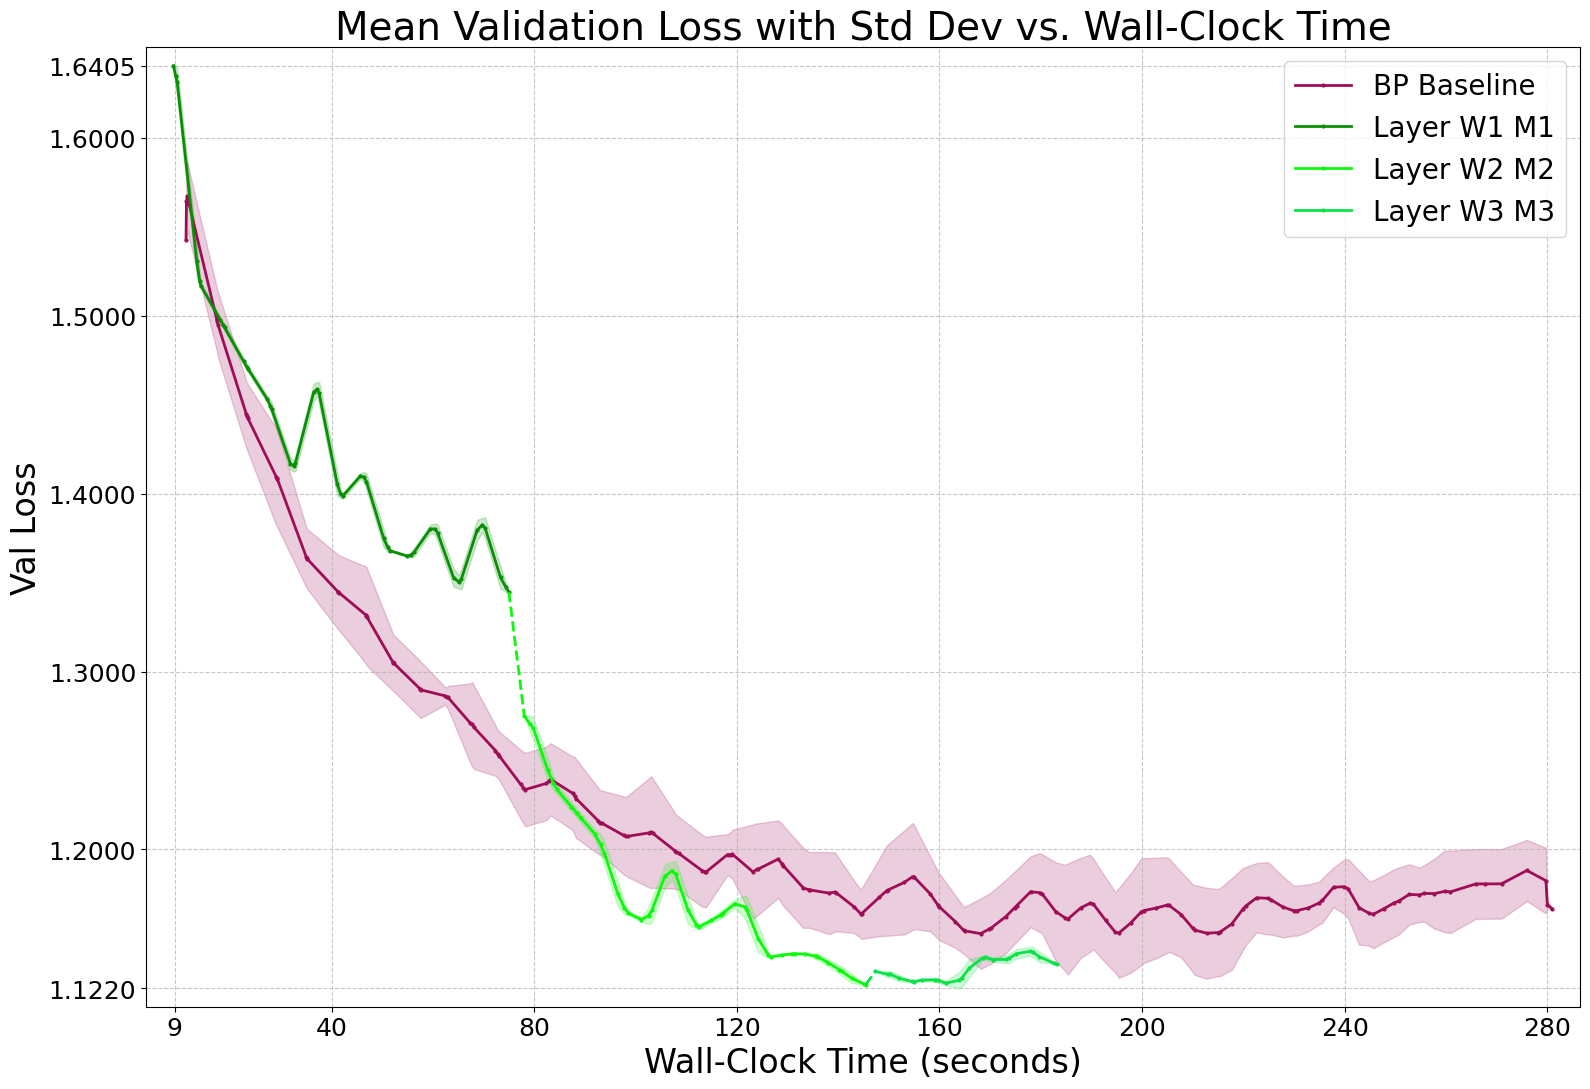
\includegraphics[width=0.9\textwidth]{plots/mf_1.png} 
    \caption{Mean Validation Loss Dynamics for MF vs. BP on CIFAR-10 3 $\times$ 2000 MLP.}
    \label{fig:mf_bp_cifar10_mlp_conv_curves}
\end{figure}

However, the most significant findings relate to MF's profound computational and energy efficiency gains. The algorithm demonstrates a marked advantage in the time required to reach its optimal validation checkpoint, proving approximately 33.8\% faster than its BP counterpart on the CIFAR-10 MLP. The combination of lower power consumption and shorter training duration results in substantial energy savings. On the CIFAR-10 task, MF consumed approximately 40.8\% less energy and produced 39.2\% less estimated CO2e than BP did, highlighting its potential, as quantified in Table~\ref{tab:mf_bp_mlp_eff_ch4}.

\begin{table}[t!] % <-- Changed from [htbp] to [t!] to encourage top placement
    \centering
    \caption{Efficiency Comparison: MF vs. BP on Native MLP Architectures (Mean ± Std Dev over 3 runs).}
    \label{tab:mf_bp_mlp_eff_ch4}
    \resizebox{\textwidth}{!}{%
    \begin{tabular}{ccc c@{ ± }c c@{ ± }c c@{ ± }c c c}
        \toprule
        Dataset & Architecture & Algorithm & \multicolumn{2}{c}{Train Time (s)} & \multicolumn{2}{c}{Energy (Wh)} & \multicolumn{2}{c}{Est. CO2e (g)} & Peak Mem (MiB) & Total GFLOPs \\
        \midrule
        \multirow{2}{*}{MNIST} & \multirow{2}{*}{2 $\times$ 1000 MLP} & MF & \textbf{35.03} & \textbf{1.51} & \textbf{0.60} & \textbf{0.03} & \textbf{1.15} & \textbf{0.08} & 934 & \textbf{0.00359} \\
        & & BP  & 39.84 & 0.20 & 0.69 & 0.00 & 1.30 & 0.04 & \textbf{926} & 0.01077 \\
        \midrule
        \multirow{2}{*}{F-MNIST} & \multirow{2}{*}{2 $\times$ 1000 MLP} & MF  & 52.08 & 0.43 & 0.86 & 0.03 & 1.64 & 0.34 & 934 & \textbf{0.00359} \\
        & & BP  & \textbf{44.06} & \textbf{4.45} & \textbf{0.79} & \textbf{0.11} & \textbf{1.62} & \textbf{0.57} & \textbf{926} & 0.01077 \\
        \midrule
        \multirow{2}{*}{CIFAR-10} & \multirow{2}{*}{3 $\times$ 2000 MLP} & MF & \textbf{177.70} & \textbf{1.62} & \textbf{3.17} & \textbf{0.06} & \textbf{6.70} & \textbf{0.71} & \textbf{1120} & \textbf{0.02833} \\
        & & BP & 268.45 & 11.47 & 5.35 & 0.22 & 11.03 & 0.45 & 1184 & 0.08499 \\
        \midrule
        \multirow{2}{*}{CIFAR-100} & \multirow{2}{*}{3 $\times$ 2000 MLP} & MF & \textbf{110.36} & \textbf{1.33} & \textbf{2.02} & \textbf{0.03} & 3.46 & 0.35 & \textbf{1142} & \textbf{0.02869} \\
        & & BP & 111.78 & 12.44 & 2.30 & 0.26 & \textbf{3.29} & \textbf{0.48} & 1192 & 0.08607 \\
        \bottomrule
    \end{tabular}%
    }
    \caption*{\footnotesize Total GFLOPs: Estimated per sample ($F_{fwd}$ for MF, $F_{BP\_update}$ for BP). Best efficiency results in each group are in \textbf{bold} (lower is better).}
\end{table}

\pagebreak
This superior efficiency is a direct consequence of its computationally lighter design. Hardware-level monitoring reveals that MF operates at a significantly lower computational intensity (9 to 11\% GPU utilization) compared to BP (16 to 17\%), a direct result of eliminating the backward pass, as seen in Figure~\ref{fig:mf_bp_gpu_util}. This reduced computational load leads to a reduced thermal profile, which is confirmed by the GPU temperature readings in Figure~\ref{fig:mf_bp_gpu_temp}. 

\begin{figure}[htbp]
    \centering
    \begin{subfigure}{1.0\textwidth}
        \centering
        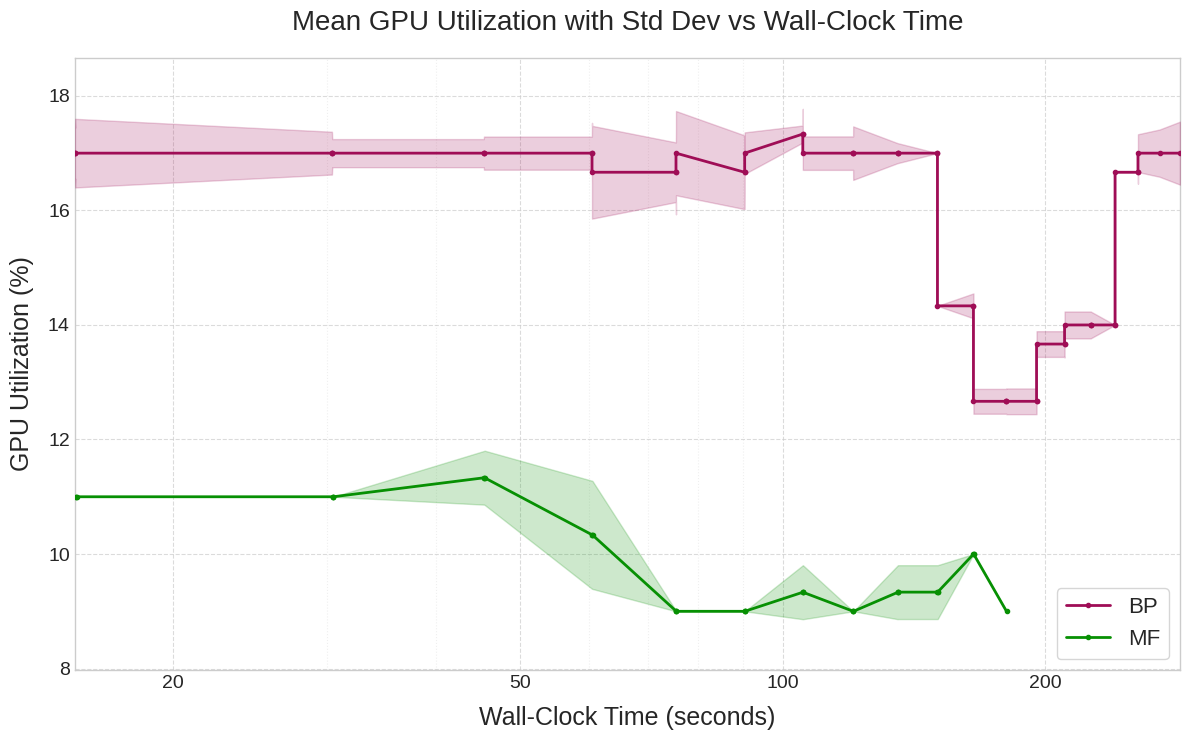
\includegraphics[width=\linewidth]{plots/mf_3.png}
        \caption{}
        \label{fig:mf_bp_gpu_util}
    \end{subfigure}
    \hfill
    \begin{subfigure}{1.0\textwidth}
        \centering
        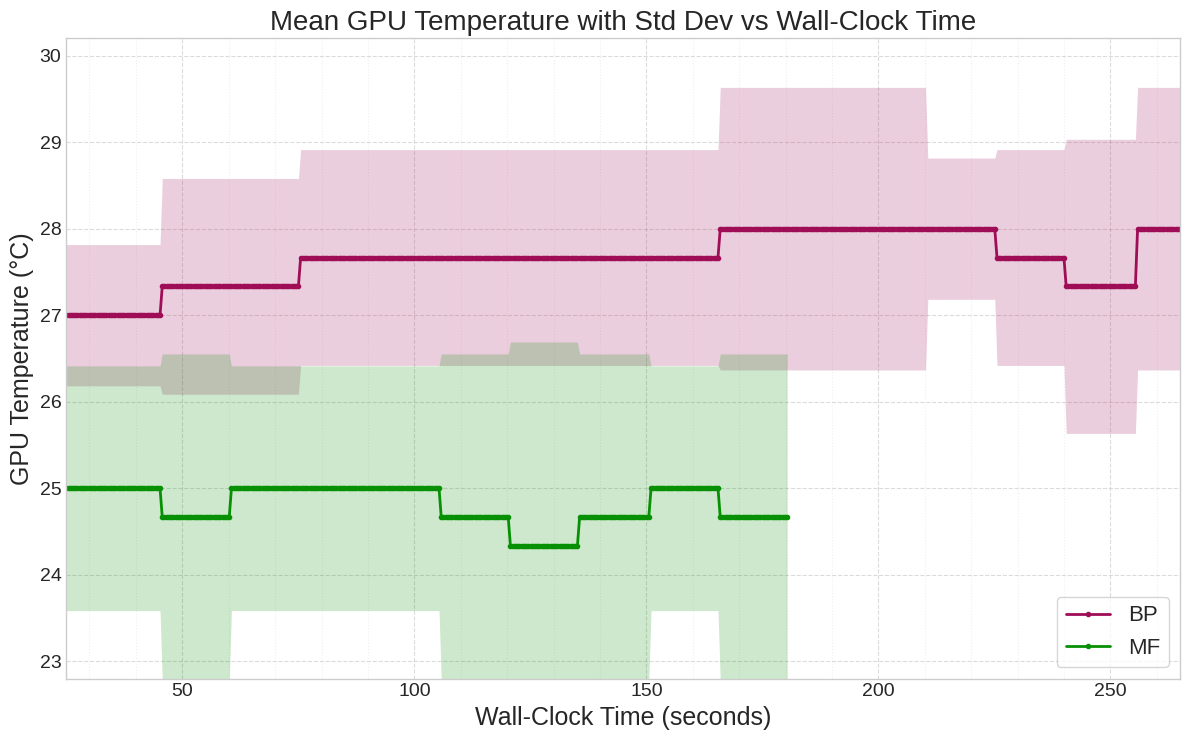
\includegraphics[width=\linewidth]{plots/mf_4.png} 
        \caption{}
        \label{fig:mf_bp_gpu_temp}
    \end{subfigure}
    \caption{Hardware-level Efficiency Indicators for MF vs. BP Training on CIFAR-10 3 $\times$ 2000 MLP.}
    \label{fig:mf_bp_hardware_indicators}
\end{figure}

Although the efficiency gains in time and energy are profound, the analysis of peak memory consumption presents a more nuanced picture. Contrary to the common expectation that BP-free methods yield large memory savings, empirical evidence shows that the MF's advantage in this domain is modest. It realizes maximum memory reductions of approximately 4 to 5\% on the larger MLPs, while incurring a slight increase on the smaller ones (Table~\ref{tab:mf_bp_mlp_eff_ch4}).

\pagebreak
This important finding highlights that the theoretical memory benefit of avoiding intermediate activation storage is partially offset by the practical memory overhead of MF's unique components: the learnable projection matrix ($\mathbf{M}_i$) associated with each layer and the memory required for its corresponding optimizer states. This result qualifies generalized claims and underscores the necessity of empirical measurement to develop a complete understanding of an algorithm's resource profile. Furthermore, the dynamic monitoring plots serve as powerful, independent signatures that validate MF's unique training mechanism is operating as designed. The dynamic memory plot in Figure~\ref{fig:mf_bp_proc_mem} provides a clear visual narrative, where the distinct step-like increase in MF's memory usage aligns perfectly with the sequential initiation of each layer's training. 

\begin{figure}[htbp]
    \centering
    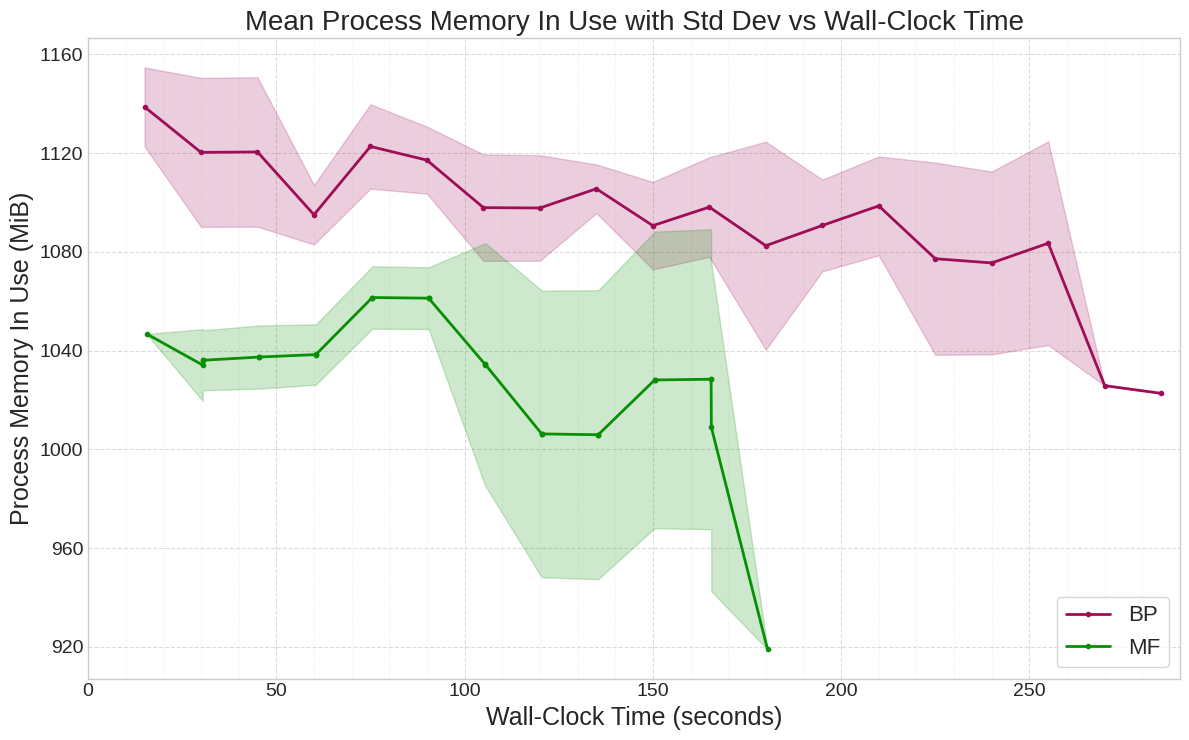
\includegraphics[width=0.99\textwidth]{plots/MF_5.png}
    \caption{Mean Process Memory In Use for MF vs. BP on CIFAR-10 3 $\times$ 2000 MLP.}
    \label{fig:mf_bp_proc_mem}
\end{figure}
\subsection{Cross Algorithm Comparative Synthesis}
\label{sec:exp_cross_algo_summary_ch4}

To synthesize the empirical findings detailed in the preceding sections, this analysis provides a consolidated overview of the performance and efficiency results across all evaluated algorithms. Table~\ref{tab:cross_algo_summary_results_ch4_updated} quantifies the relative differences between each alternative training method and its corresponding fair backpropagation baseline, calculated from the mean results of three experimental runs. This comparative summary enables a direct assessment of the trade-offs inherent in each approach when implemented on its native architecture.

\begin{table}[t!]
    \centering
    % Setup for siunitx columns
    \sisetup{
        table-format = +4.2,      % Format: sign, up to 4 digits before decimal, 2 after
        retain-explicit-plus,     % Show the '+' sign when present
        table-align-text-post = false % Align numbers, not the text after them
    }
    \caption{Relative Performance and Efficiency Summary vs. Fair BP Baselines (Mean over 3 runs).}
    \label{tab:cross_algo_summary_results_ch4_updated}
    \resizebox{\textwidth}{!}{%
    % Use the S column type for numerical columns
 \begin{tabular}{>{\centering\arraybackslash}m{3.2cm} l >{\centering\arraybackslash}m{2.8cm} S S S S}
        \toprule
        % THE FIX: Wrap the headers of the S columns in braces {}
        Algorithm Variant & Dataset & Architecture & {$\Delta$ Acc. (\%)} & {$\Delta$ Time (\%)} & {$\Delta$ Energy (\%)} & {$\Delta$ Mem. (\%)} \\
        \midrule
        FF-AdamW & F-MNIST & MLP 4 $\times$ 2000 & +0.75 & +1233.26 & +862.35 & +1.88 \\
        FF-AdamW & MNIST & MLP 3 $\times$ 1000 & +0.24 & +342.11 & +339.95 & +0.85 \\
        FF-SGD & MNIST & MLP 3 $\times$ 1000 & +0.14 & +429.69 & +419.67 & +1.06 \\
        FF-AdamW & MNIST & MLP 4 $\times$ 2000 & -0.01 & +305.08 & +236.88 & +1.88 \\
        \midrule
        CaFo-Rand-CE & MNIST & CNN 3-block& -0.32 & +88.48 & +32.65 & -6.67 \\
        CaFo-DFA-CE & MNIST & CNN 3-block& +0.08 & +124.82 & +81.83 & +1.11 \\
        \cmidrule(lr){2-7}
        CaFo-Rand-CE & F-MNIST & CNN 3-block& +1.11 & +205.00 & +115.99 & -6.67 \\
        CaFo-DFA-CE & F-MNIST & CNN 3-block& \bfseries +2.47 & +206.51 & +201.43 & +1.11 \\
        \cmidrule(lr){2-7}
        CaFo-Rand-CE  & CIFAR-10 & CNN 3-block& -13.23 & -2.96 & -19.24 & \bfseries -8.98 \\
        CaFo-DFA-CE & CIFAR-10 & CNN 3-block& -1.72 & +287.17 & +301.94 & +1.26 \\
        \cmidrule(lr){2-7}
        CaFo-Rand-CE  & CIFAR-100 & CNN 3-block& -11.44 & +246.27 & +188.87 & -5.02 \\
        CaFo-DFA-CE & CIFAR-100 & CNN 3-block& -4.43 & +557.19 & +576.82 & +2.51 \\
        \midrule
        MF & MNIST & MLP 2 $\times$ 1000 & +0.09 & -12.07 & -13.34 & +0.86 \\
        MF  & F-MNIST & MLP 2 $\times$ 1000 & +0.51 & +18.20 & +9.90 & +0.86 \\
        MF  & CIFAR-10 & MLP 3 $\times$ 2000 & +1.21 & \bfseries -33.81 & \bfseries -40.78 & -5.41 \\
        MF  & CIFAR-100 & MLP 3 $\times$ 2000 & +0.37 & -1.28 & -12.48 & -4.19 \\
        \bottomrule
    \end{tabular}%
    }
    \caption*{\footnotesize The metric $\Delta$ represents the difference between the alternative algorithm and its fair BP baseline. A positive $\Delta$Acc. is better. Negative values for other metrics are better. The \textbf{bold} values highlight the best in class improvement for each metric across all experiments and algorithms.}
\end{table}

The results consolidated in Table~\ref{tab:cross_algo_summary_results_ch4_updated} crystallize the main findings of this chapter. The Forward-Forward algorithm proved to be prohibitively inefficient, despite validating the foundational premise of BP-free learning by achieving an accuracy comparable to that of backpropagation on MLPs. Its training time and energy costs were consistently and substantially higher, without realizing any peak memory advantage in these experiments. The Cascaded-Forward algorithm, evaluated on its native CNNs, revealed a nuanced performance profile contingent on its implementation variant. The CaFo-Rand-CE variant demonstrated modest efficiency gains, including a notable 19.2\% energy reduction and a 9.0\% memory reduction on the CIFAR-10 task, but at the cost of a significant 13.23 percentage point decrease in accuracy.

In contrast, the CaFo-DFA-CE variant substantially improved accuracy, even surpassing BP on less complex datasets, yet the resource-intensive DFA pre-training phase led to profoundly greater time and energy consumption. Lastly, the Mono-Forward algorithm, when evaluated on its native MLP architectures, consistently presented the most compelling profile among the investigated alternatives. Not only did it achieve accuracy parity or superiority over its BP baselines, but it also delivered substantial reductions in training time and energy consumption, particularly on more complex datasets. The peak memory savings, while more modest, were consistent for the larger MLP architectures.

In aggregate, the experimental findings of this chapter chart an evolutionary progression from a conceptually significant but practically inefficient algorithm (FF), through a structured method defined by acute trade-offs (CaFo), to a highly promising algorithm (MF) that, within the domain of MLP architectures, effectively synthesizes superior accuracy with superior training efficiency. This empirical evidence provides the foundation for the critical analysis of algorithmic mechanisms and practical implications presented in the subsequent chapter.